

\tikzset{every picture/.style={line width=0.75pt}} %set default line width to 0.75pt        

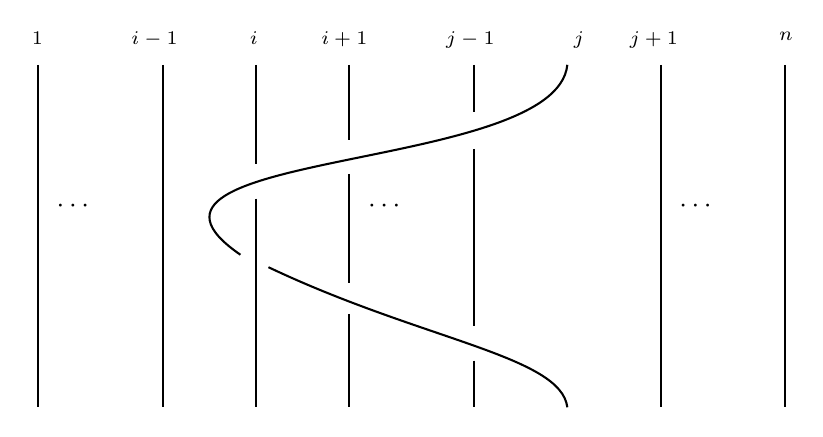
\begin{tikzpicture}[x=0.75pt,y=0.75pt,yscale=-1.5,xscale=1.5]
%uncomment if require: \path (0,877); %set diagram left start at 0, and has height of 877

%Straight Lines [id:da43079767492294996] 
\draw    (100,40) -- (100,150) ;
%Straight Lines [id:da8568972494568349] 
\draw    (140,40) -- (140,150) ;
%Straight Lines [id:da39499802412559726] 
\draw    (170,40) -- (170,72) ;
%Straight Lines [id:da06352980068118319] 
\draw    (200,40) -- (200,64) ;
%Straight Lines [id:da5832724793835432] 
\draw    (240,40) -- (240,55) ;
%Straight Lines [id:da9487132303393538] 
\draw    (300,40) -- (300,150) ;
%Straight Lines [id:da2547896303322166] 
\draw    (340,40) -- (340,150) ;
%Curve Lines [id:da9573368491042561] 
\draw    (270,40) .. controls (266.5,75) and (115.5,67) .. (165,101) ;
%Straight Lines [id:da3325229398873272] 
\draw    (170,83) -- (170,150) ;
%Curve Lines [id:da11849363606307461] 
\draw    (174,105) .. controls (223.5,128.5) and (268,133.5) .. (270,150) ;
%Straight Lines [id:da16906643654568176] 
\draw    (200,75) -- (200,110) ;
%Straight Lines [id:da11587080674469141] 
\draw    (200,120) -- (200,150) ;
%Straight Lines [id:da014801284669030856] 
\draw    (240,67) -- (240,124) ;
%Straight Lines [id:da15561552279853996] 
\draw    (240,135) -- (240,150) ;

% Text Node
\draw (105,82.4) node [anchor=north west][inner sep=0.75pt]    {$\cdots $};
% Text Node
\draw (205,82.4) node [anchor=north west][inner sep=0.75pt]    {$\cdots $};
% Text Node
\draw (305,82.4) node [anchor=north west][inner sep=0.75pt]    {$\cdots $};
% Text Node
\draw (97,28.4) node [anchor=north west][inner sep=0.75pt]  [font=\scriptsize]  {$1$};
% Text Node
\draw (129,28.4) node [anchor=north west][inner sep=0.75pt]  [font=\scriptsize]  {$i-1$};
% Text Node
\draw (167,28.4) node [anchor=north west][inner sep=0.75pt]  [font=\scriptsize]  {$i$};
% Text Node
\draw (190,28.4) node [anchor=north west][inner sep=0.75pt]  [font=\scriptsize]  {$i+1$};
% Text Node
\draw (230,28.4) node [anchor=north west][inner sep=0.75pt]  [font=\scriptsize]  {$j-1$};
% Text Node
\draw (271,28.4) node [anchor=north west][inner sep=0.75pt]  [font=\scriptsize]  {$j$};
% Text Node
\draw (289,28.4) node [anchor=north west][inner sep=0.75pt]  [font=\scriptsize]  {$j+1$};
% Text Node
\draw (337,28.4) node [anchor=north west][inner sep=0.75pt]  [font=\scriptsize]  {$n$};


\end{tikzpicture}
